\documentclass[12pt]{article}

\usepackage{geometry}
\usepackage[utf8]{inputenc}
\usepackage[polish]{babel}
\usepackage{polski}
\usepackage{hyperref}
\usepackage{graphicx}
\usepackage{verbatim}
\usepackage{acronym}
\usepackage{fancyhdr}
\usepackage[usenames]{color}
\definecolor{linkcolor}{rgb}{0.5, 0.15, 0.15}

\hypersetup{
  linkbordercolor={1 1 1},
  urlbordercolor={1 1 1},
  linkcolor=linkcolor,
  colorlinks=true
}

\pagestyle{fancy}
\cfoot{}
\rfoot{\thepage}

\author{Michał Bugno \and Antek Piechnik}
\title{Analiza oraz wizualizacja danych meteorologicznych dla wybranych ośrodków narciarskich}
% W oparciu o bazę danych Oracle z wykorzystaniem technologii Oracle Spatial.

\begin{document}
\maketitle
\tableofcontents
\newpage

\section{Wizja projektu}
Głównym zadaniem projektu jest dogłębne poznanie struktury
danych typu GIS (geographical information system), jak również analiza oraz
wykorzystanie tego typu danych w wizualizacji danych meteorologicznych. System
docelowo ma za zadanie przedstawienie sytuacji meteorologicznej na podstawie
danych zbieranych na bieżąco jak również danych historycznych zebranych
poprzednio. System ma również mieć możliwość udostępniania danych/wizualizacji
historycznych na życzenie użytkownika. Do celów badania wydajności systemu
wykorzystywane będą dane z przynajmniej dwóch źródeł informacji
meteorologicznej, podczas gdy system ma domyślnie obsługiwać 4-5 stacji
narciarskich.

\section{Ogólna struktura systemu}

\subsection{Baza danych}
Wybraną bazą danych jest Oracle. Wyboru dokonaliśmy głównie ze względu na
możliwość dokładnego poznania tego produktu w ramach projektu jak również ze
względu na obszerne wsparcie (dedykowany silnik?) dla danych GIS - Oracle
Spatial.

\subsection{Aplikacja pobierająca dane z internetu (crawler)}
Aplikacja będzie w rzeczywistości skryptem mającym na celu pobranie
odpowiednich danych z wcześniej przygotowanych źródeł (stron internetowych
    udostępniających informacje meteorologiczne dla konkretnych ośrodków).
Będzie on miał również możliwość aktualizowania bazy danych o pobrane
informacje, po uprzednich skonwertowaniu ich do odpowiedniego formatu.

\subsection{Kontroler analizy danych meteorologicznych}
Kontroler analizy danych będzie odpowiadał na poszczególne wywołania i na
podstawie analizy danych zebranych w bazie stworzy zestaw informacji
potrzebnych do wizualizacji żądanego stanu pogodowego (obecnego lub
    historycznego).

\subsection{Renderer graficzny}
Renderer zostanie utworzony w oparciu o dane wygenerowane przez kontroler
analizy danych oraz o API systemu Google Maps który pozwoli na estetyczną
wizualizację osiągniętych wyników analizy.

\subsection{Aplikacja udostępniająca wizualizacje}
Aplikacja utworzona będzie jako aplikacja sieciowa dostępna z poziomu
przeglądarki internetowej.

\section{Architektura systemu}

Do implementacji systemu posłużymy się:
\begin{itemize}
\item językami skryptowymi - Ruby (do implementacji crawlera, części aplikacji
    webowej oraz renderera) i Python (do sprawnej komunikacji z API Google
      Maps)
\item frameworkiem aplikacji web -- Merb
\end{itemize}


\section{Przepływ danych w systemie}
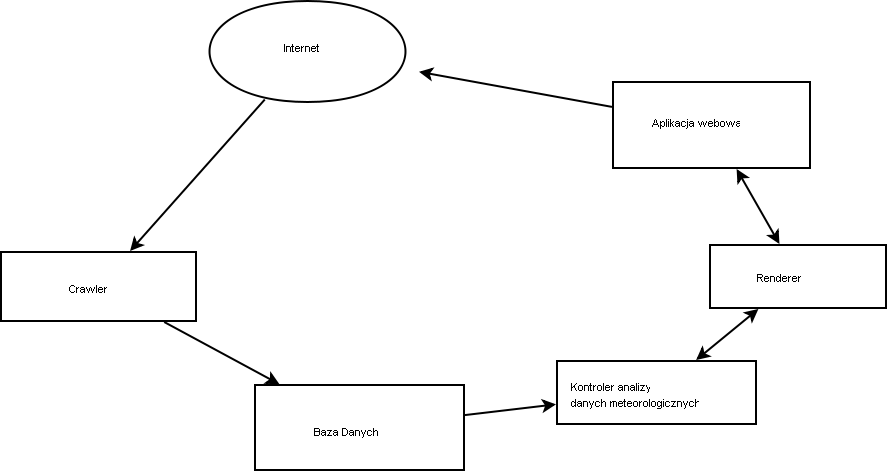
\includegraphics[width=35em]{images/data_flow_diagram.png}

\section{Baza danych}
Do momentu ustabilizowania bazy danych Oracle na serwerze AGH będziemy starali
się pracować na dostępnych za darmo silnikach typu Oracle Express (XE)
  postawionych na lokalnych maszynach, z uwzględnieniem możliwości
  przystosowania na nich aplikacji sprawnej w pełnej wersji Oracle. Wstępnie w
  bazie danych planujemy istnienie następujących danych:
\subsection{Dane informacyjne dla punktow pomiarowych.}
\begin{itemize}
  \item Nazwa Ośrodka
  \item Adres
  \item Dane GPS (no bo w sumie czemu nie, zawsze fajnie takie cos wyświetlić)
  \item Kraj
  \item Np. ilość stoków w danym ośrodku, na danej wysokości etc.
  \item Dane GIS - jakis klucz do osobnej tabeli , w której bedzie:
  \end{itemize}
\subsection{Dane GIS}
Struktura tej części danych będzie silnie uzależniona od dostępnych danych na temat (dla każdego punktu):
\begin{itemize}
  \item Wysokosci
  \item Obszaru pokrywanego pomiarami.
  \item Wspolrzednych punktu pomairowego
\end{itemize}
\subsection{Dane pomiarów}
\begin{itemize}
  \item Numer Pomiaru (klucz główny)
  \item Nazwa Punktu Pomiarowego lub klucz obcy do Danych Informacyjncyh
  \item godzina
  \item data
\end{itemize}
\subsection{Dane wartośći pomiarów}
  \begin{itemize}
  \item Numer pomiaru
  \item Temperatura max
  \item Temperatura min
  \item Wiatr- kierunek
  \item Wiatr- siła
  \item Zachmurzenie
  \item Opady sniegu
  \item Opady deszczu
\end{itemize}

\section{Crawler}
Crawler jest napisany w języku Ruby i służy do pobierania danych ze strony \url{http://www.snow-forecast.com}.
Docelowo będzie to prosty skrypt oparty o metodologię \emph{Extract--Transform--Load}. W tej chwili zaimplementowana
jest część \emph{Extract}:
\begin{itemize}
\item uruchamiamy skrypt z parametrem adresu strony (w zasadzie chodzi o wybrany szczyt)
\item skrypt analizuje stronę za pomocą parsera HTML+XML Nokogiri
\item dane zapisywanę są w prostej postaci w tablicy
\item skrypt znajduje link do danych z poprzedniego okresu, odwiedza go i powtarza proces
\end{itemize}

Dane są zapisywane w tej chwili w bardzo prostym formacie, część \emph{Transform} będzie odpowiedzialna
za konwersji ich do formatu odpowiedniego dla bazy danych

\end{document}
